Для экспериментальных исследований были необходимы данные двух типов: последовательности РНК для подачи на вход синтаксическому анализатору и эталонные вторичные структуры для этих последовательностей --- и то, и другое было получено из популярной в исследовательских работах базы данных RNAstrand~\cite{andronescu2008rna}. Эта база представляет собой сборку тщательно отобранных и приведенных к единому формату данных сразу из нескольких надежных баз, содержащих цепочки РНК вместе с полученными методами лабораторного эксперимента или эволюционного анализа вторичными структурами. Из выгруженных данных были удалены дубликаты и образцы с неточностями в нуклеотидной цепи или же вторичной структуре, а также было выставлено ограничение на максимальную длину последовательности --- таким образом была получена выборка из 801 последовательности длин от 8 до 100, для которой были сгенерированы матрицы разбора и матрицы контактов, переведенные в черно-белые изображения. Для цепочки длины $n$ и входное, и эталонное изображения имеют размер $n \times n$, поэтому для корректной обработки изображений разного размера перед каждой эпохой обучения нейросети данные группировались по батчам, в каждом из которых присутствовали изображения только одного размера. Если количество образцов какого-либо размера оказывалось меньше величины batch size или же не делилось на него нацело, данные циклическим образом дублировались до достижения необходимого объема. Распределение длин последовательностей в итоговой выборке продемонстрировано на рис.~\ref{plot_distr}, при этом медианным значением является 44, а средним --- 47, что говорит о практически одинаковой представленности коротких и длинных цепочек среди исследуемых данных.

\begin{figure}[h]
\begin{center}
\centering

\includegraphics[width=14.5cm]{pics/plot_distr.png}
\caption{Распределение длин последовательностей РНК в выборке}
\label{plot_distr}
\end{center}
\end{figure} 

Для оценки качества работы обученных на данных изображениях нейронных сетей были выбраны следующие метрики, посчитанные относительно попиксельной разницы между предсказанным и эталонным изображениями. Далее $TP$ (true positive), $FP$ (false positive) и $FN$ (false negative), где под positive и negative  понимаются белые и черные пиксели изображений соответственно, --- информация о том, сколько раз нейронная сеть приняла верное и сколько раз неверное решение по каждому пикселю (кроме диагональных) каждого изображения выборки.
\begin{itemize} 
    \item $Precision = \frac{TP}{TP + FP}$ (доля предсказанных контактов, которые действительно являются контактами в эталонном изображении).
    \item $Recall = \frac{TP}{TP + FN}$ (доля найденных нейронной сетью контактов среди всех искомых).
    \item $F1 = 2 * \frac{Precision * Recall}{Precision + Recall}$ (гармоническое среднее $Precision$ и $Recall$, используется как удобная объединяющая метрика).
\end{itemize}

При обучении нейросети была использована функция потерь, в основе построения которой лежит идея о максимизации метрики $F1$ с несколькими уточнениями. Во-первых, $F1$ дискретна, а функция ошибки должна быть дифференцируема вследствие вычисления на ней градиента. Во-вторых, передача среднего по выборке значения $1 - F1$ в качестве функции ошибки не гарантирует отсутствие большого разброса $Precision$ и $Recall$ как в пределах отдельно взятого изображения, так и в масштабах всей выборки, следствием чего будет нестабильность качества работы модели и высокая вероятность появления очень низкой точности результата для случайно взятого тестового образца. На основании данных соображений была реализована функция $F1\_loss$, представленная на рис.~\ref{loss}. Здесь дифференцируемость обеспечивается заменой сумм дискретных целочисленных значений на непрерывную сумму значений вероятности, а поддержка баланса между $Precision$ и $Recall$ для каждого изображения и для выборки в целом --- двумя пропорциональными величине разброса штрафными коэффициентами $k1$ и $k2$, накладываемыми на метрику $F1$.

\begin{figure}[h]
\begin{center}
\centering
\begin{python}
from keras import backend as K

def f1_loss(y_true, y_pred):
    #normalize pixels values to [0, 1]
    y_true, y_pred = K.minimum(y_true / 255, 1), K.minimum(y_pred / 255, 1)
    #calculate differentiable versions of TW, FW and FB
    tw = K.sum(K.cast(y_true * y_pred, 'float32'), axis=[1, 2, 3])
    fw = K.sum(K.cast((1 - y_true) * y_pred, 'float32'), axis=[1, 2, 3])
    fb = K.sum(K.cast(y_true * (1 - y_pred), 'float32'), axis=[1, 2, 3])
    #calculate precision and recall secure from zero division error
    precision = tw / (tw + fw + K.epsilon())
    recall = tw / (tw + fb + K.epsilon())
    #penalty coefficients for huge difference between precision and recall 
    #calculated for each image and whole dataset respectively
    k1 = 1 -  K.abs(precision - recall)
    k2 = 1 -  K.abs(K.mean(precision) - K.mean(recall))
    #calculate upgraded f1 score
    f1 = k1 * k2 * 2 * precision * recall / (precision + recall + K.epsilon()) 
    return 1 - K.mean(f1)
\end{python}
\caption{Функция потерь нейронной сети}
\label{loss}
\end{center}
\end{figure} 

Вследствие того, что количество обучаемых параметром используемой модели является достаточно большим относительно размера выборки, после каждого остаточного блока был добавлен слой Dropout, исключающий заданный процент случайных нейронов во время обучения. Кроме того, во всех сверточных слоях была применена регуляризация L2, которая, помимо уменьшения переобучения нейросети, оказывает положительное влияние на процесс поиска сложных закономерностей в данных. В качестве оптимизатора был использован адаптивный градиентный спуск (Adagrad)~\cite{duchi2011adaptive}, удобный для работы с разреженными данными, а также автоматически настраивающий скорость обучения.

Для сравнения результатов работы обученной модели с существующими в области аналогами был проведен анализ различных инструментов, предсказывающих вторичную структуру РНК, по следующим критериям: заявленная высокая точность результатов, возможность предсказания псевдоузлов, удобство использования и адекватное время работы. На основании данных соображений были отобраны шесть инструментов, основанных на различных подходах.
\begin{itemize}
    \item HotKnots --- минимизации свободной энергии через эвристический алгоритм~\cite{ren2005hotknots}.
    \item SPOT-RNA --- глубокое обучение, основанное на технике transfer learning~\cite{singh2019rna}.
    \item PknotsRG --- минимизация свободной энергии с использованием Turner energy rules~\cite{reeder2007pknotsrg}.
    \item RNAstructure --- минимизация свободной энергии с помощью динамического программирования~\cite{bellaousov2013rnastructure}.
    \item Ipknot --- поиск оптимальной вторичной структуры методом целочисленного программирования~\cite{sato2011ipknot}.
    \item Knotty --- алгоритм для минимизация свободной энергии, основанный на разреженном динамическом программировании~\cite{jabbari2018knotty}.
\end{itemize}

\subsection{Результаты}
Все тестовые запуски проводились на рабочей станции со следующими характеристиками.
\begin{itemize}
    \item Операционная система: Ubuntu 20.04.2 LTS.
    \item Центральный процессор: Intel Core i5-10210U CPU 1.60GHz.
    \item Графический процессор: NVIDIA GeForce MX250.
    \item Объем оперативной памяти: 7.5 GB.
\end{itemize}

На рис.~\ref{plot_f1} представлены значения метрики $F1$, показанные шестью вышеописанными инструментами на всей выборке из 801 образца, а разработанной моделью (New-model) --- для различных разделений данных на обучающую и тестовую выборки (10\%:90\%, ..., 90\%:10\%). На графике видно, что при малых размерах обучающей выборки новая модель демонстрирует достаточно низкую точность, однако при увеличении выборки до 40\% результаты становятся сравнимыми с остальными подходами, а при максимальном объеме выборки (90\%) ---  лучшими в приведенном сравнении.

На рис.~\ref{plot_pr} показаны результаты аналогичного тестирования всех моделей по метрикам $Precision$ и $Recall$; здесь черная прямая $y=x$ символизирует оптимальное для рассматриваемой задачи положение этих метрик --- их равенство, --- а фиолетовая пунктирная линия указывает направление увеличения размера обучающей выборки для нашей модели от 10\% до 90\% с шагом в 10\%. Значения метрик для New-model расположены достаточно близко к желаемой прямой, что говорит о сбалансированности предсказаний разработанной нейросети. Кроме того, реализованный в данной работе алгоритм --- единственный на данном графике, имеющий $Recall$, больший, чем $Precision$: это произошло из-за того, что парсер находит значительную часть требуемых контактов, поэтому нейронная сеть, владея этой информацией еще до начала обучения, основной своей задачей имеет улучшение точности, а не полноты системы. Это делает наш подход несколько нетрадиционным относительно аналогов, которые, по всей видимости, сталкиваются с рядом проблем в процессе поиска контактов во вторичной структуре.

\begin{figure}[h]
\centering
\begin{subfigure}{.5\textwidth}
  \centering
  \fbox{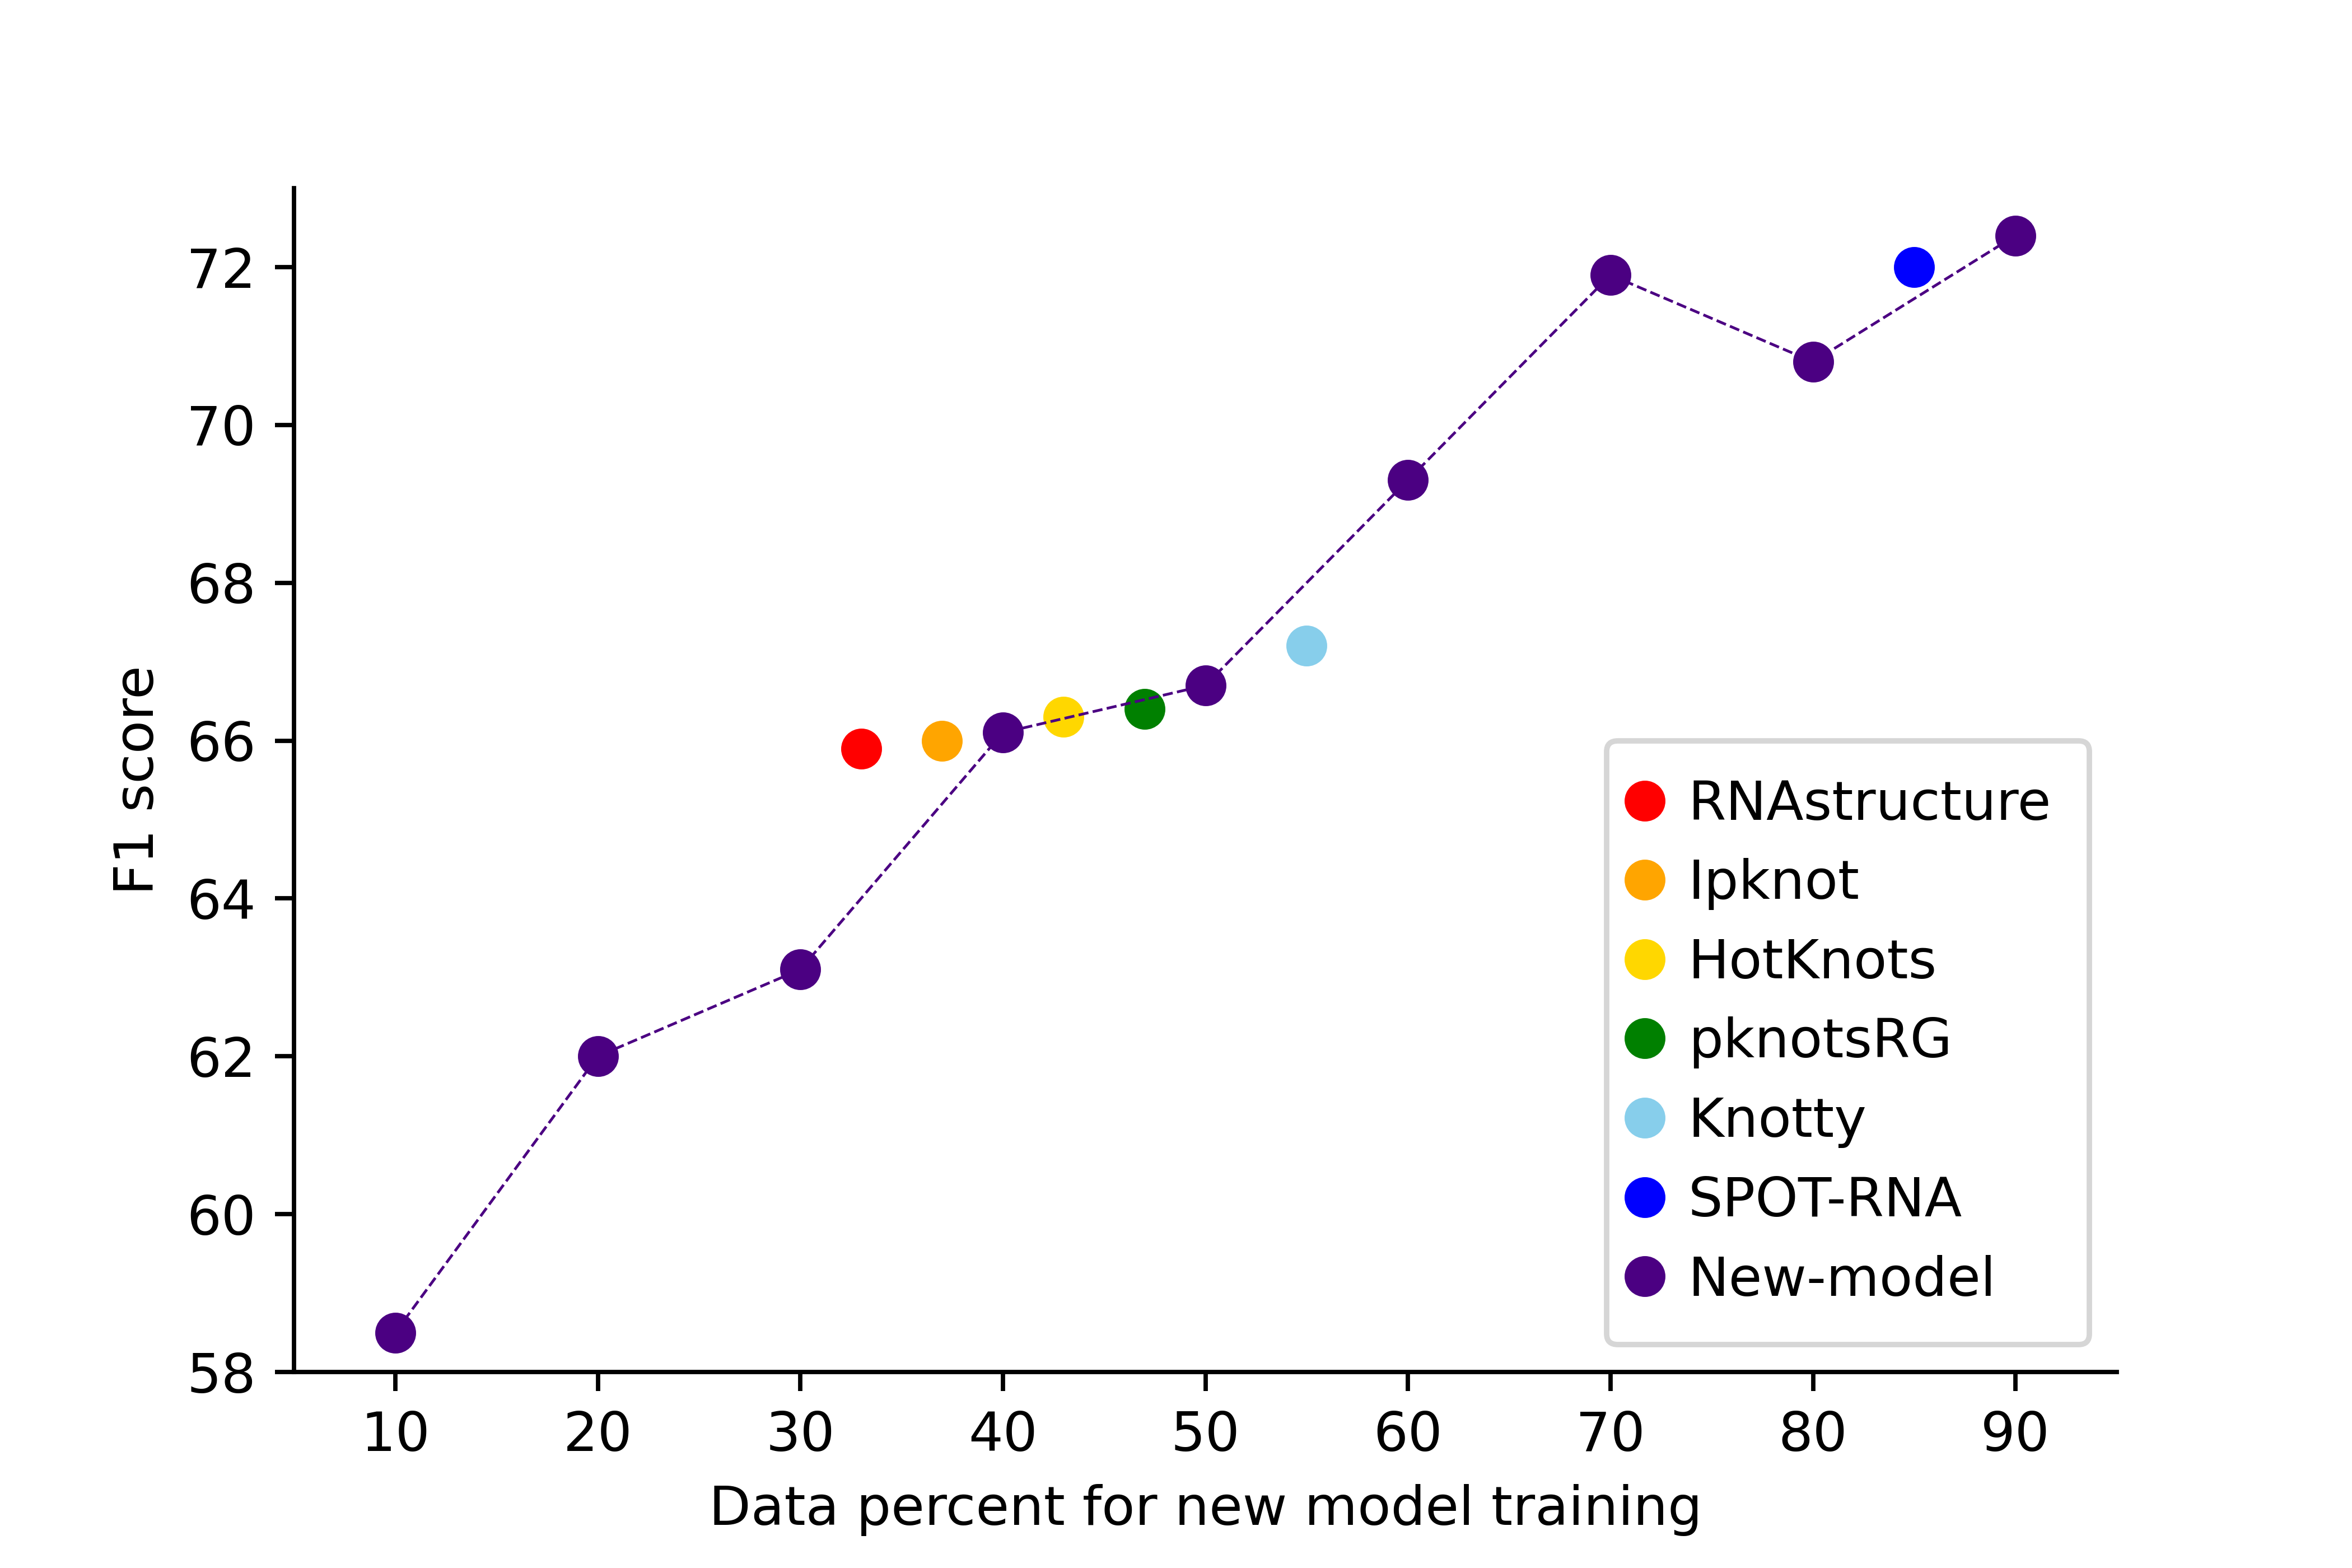
\includegraphics[width=.95\linewidth]{pics/plot_f1.png}}
  \caption{Значения метрики $F1$}
  \label{plot_f1}
\end{subfigure}%
\begin{subfigure}{.5\textwidth}
  \centering
  \fbox{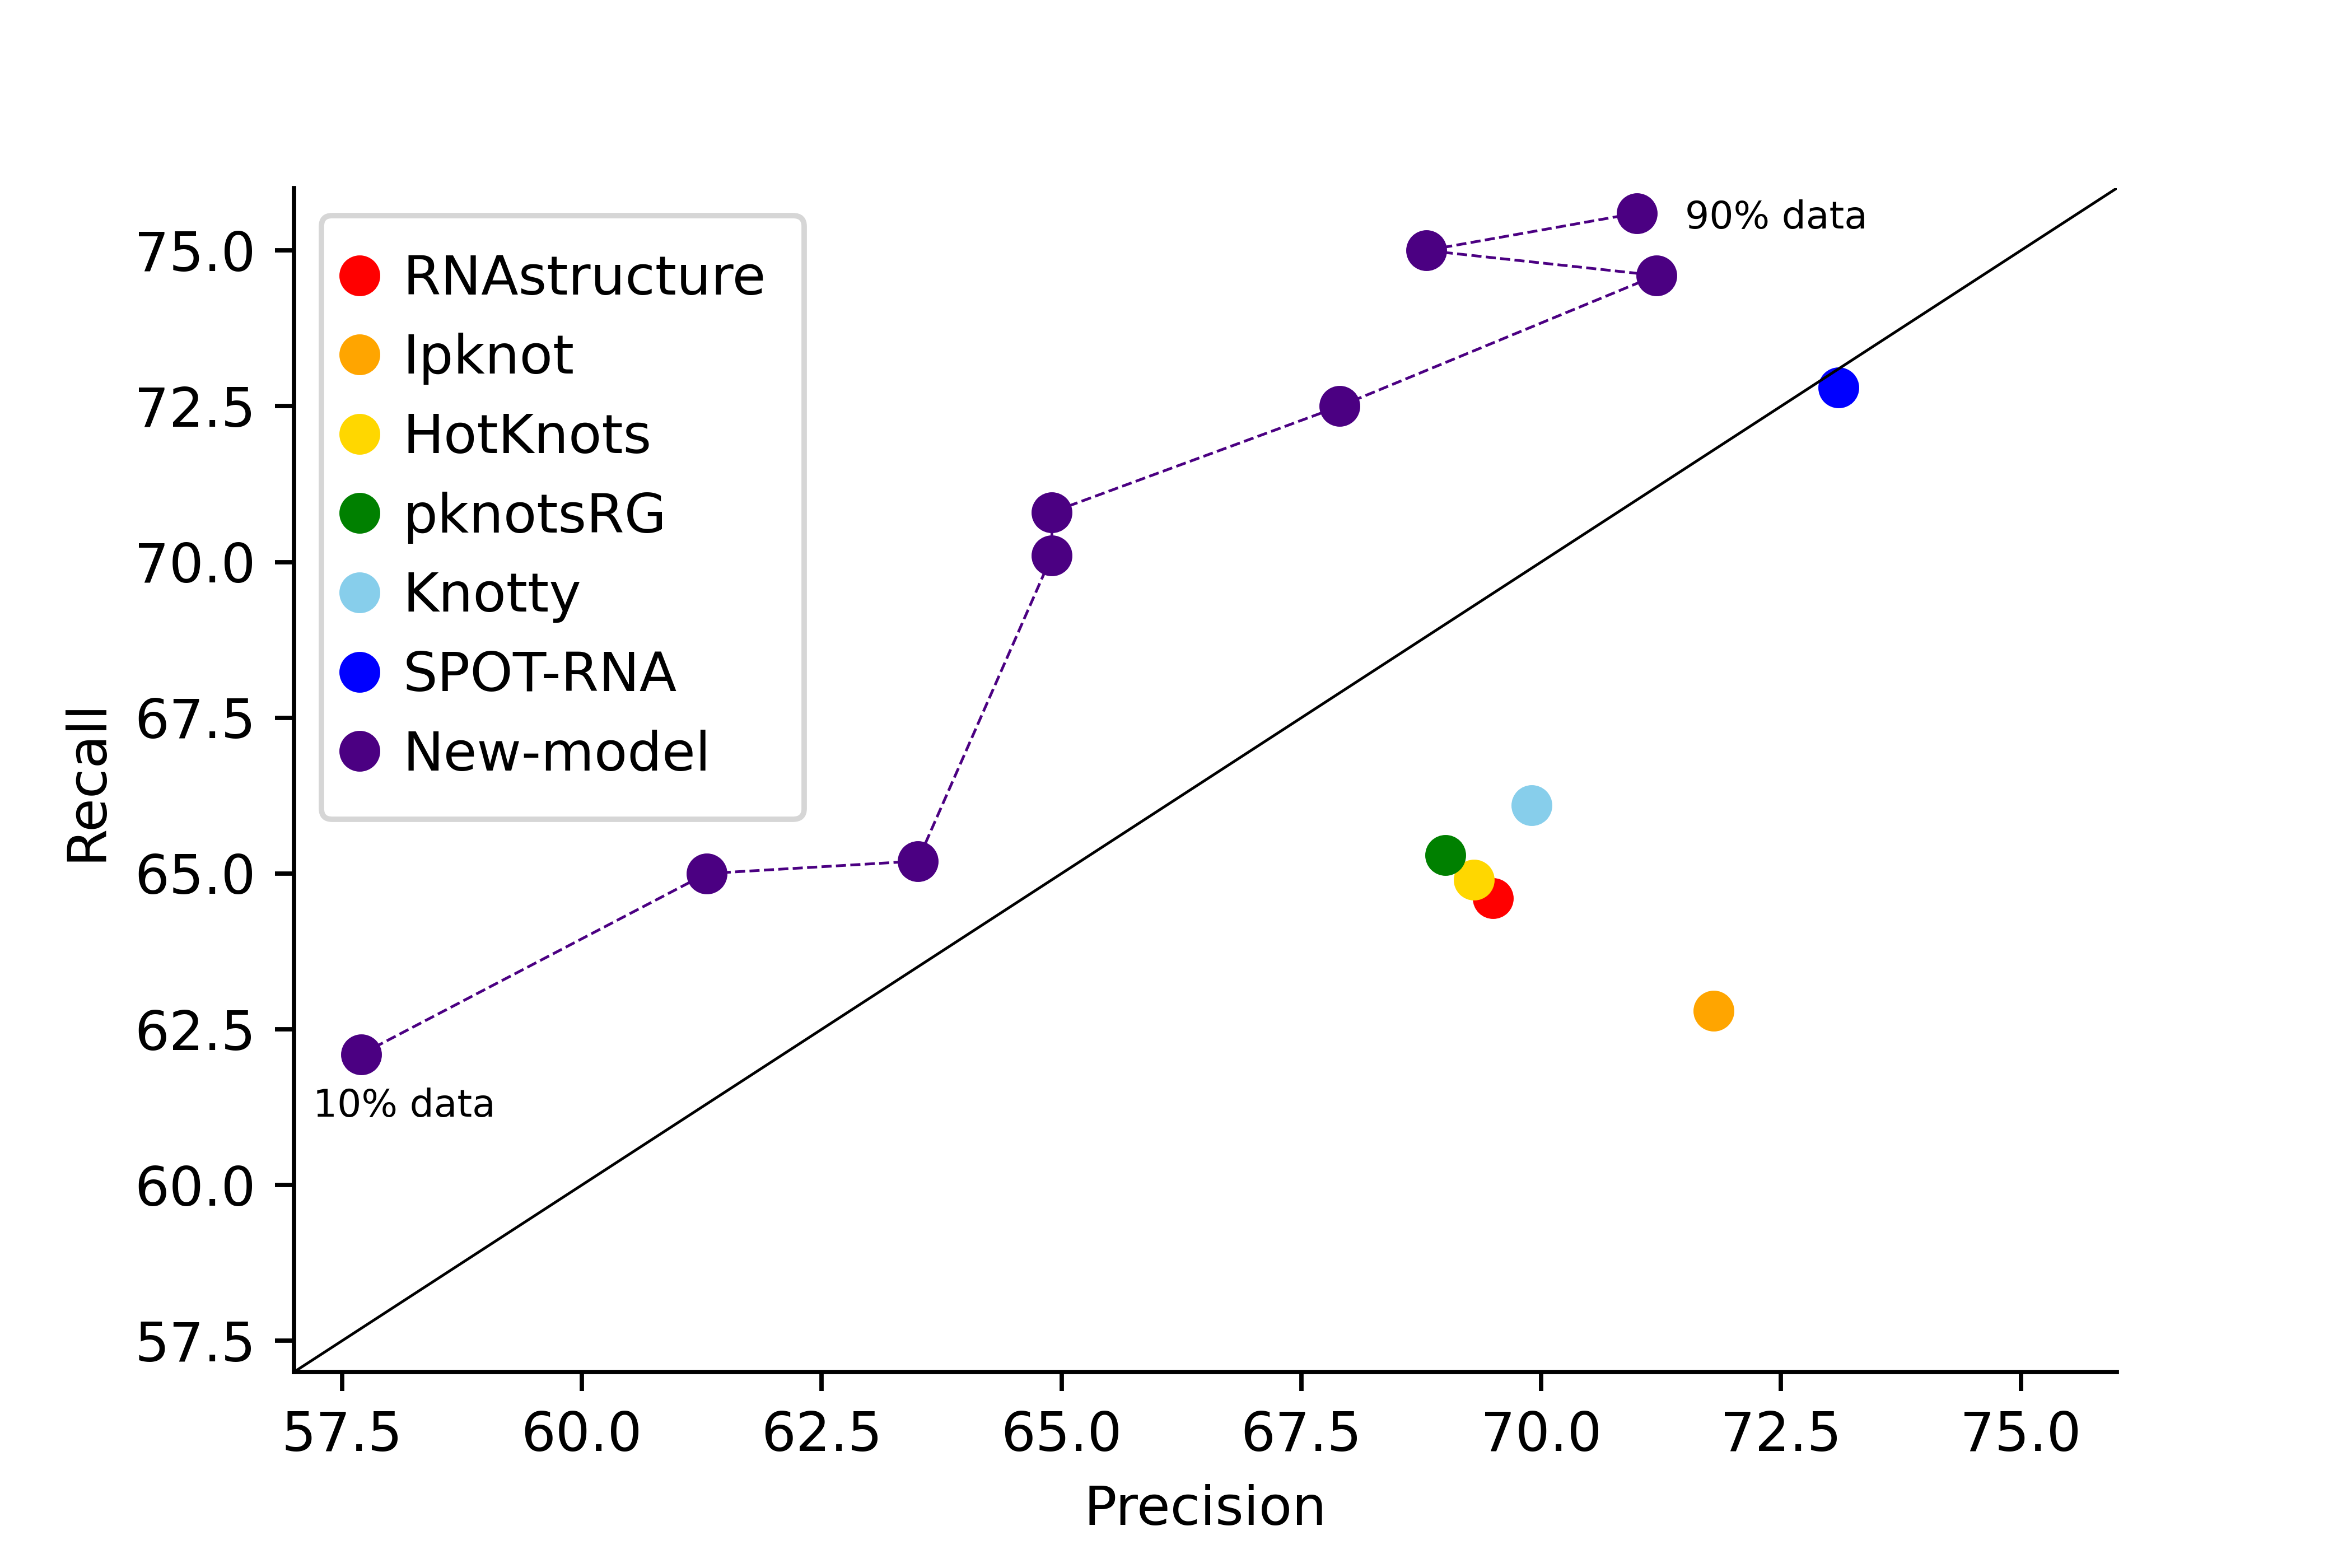
\includegraphics[width=.95\linewidth]{pics/plot_pr.png}}
  \caption{Значения метрик $Precision$ и $Recall$}
  \label{plot_pr}
\end{subfigure}
\caption{Сравнение разработанного подхода с аналогами}
\label{plot}
\end{figure}

Помимо точности, важной характеристикой алгоритма в области биоинформатики является время его работы, так как исследователям часто приходится работать с достаточно большими биологическими базами данных. В таблице~\ref{time} приведены замеры времени, потраченного всеми инструментами на обработку 100 цепочек РНК различных длин из рассматриваемого промежутка от 8 до 100. Несмотря на то, что разные подходы могут предполагать разные сценарии использования (обработка одной или нескольких последовательностей, вывод ответа через интерфейс командной строки или в специальный файл, а также сохранение результатов в различных форматах), одним из традиционных вариантов является обработка файла в формате fasta, содержащего набор последовательностей с метаданными, и последующее сохранение результата в одном из общепринятых форматов (например, dot-bracket или bpseq). Для данного сценария и был произведен сравнительный анализ производительности подходов: файл с последовательности был преобразован в необходимые для всех инструментов входные форматы, выходные же форматы были оставлены без изменений. В таблице~\ref{time} представлены средние значения для десяти прогонов в секундах, упорядоченные по возрастанию времени. Инструменты Ipknot, Hotknots, PknotsRG, RNAstructure и Knotty работают только на CPU, SPOT-RNA имеет и CPU, и GPU-реализации, а для нашего подхода как алгоритм синтаксического анализа (PA), так и нейронная сеть (NN) используют GPU. Можно увидеть, что New-model значительно проигрывает по времени большинству аналогов и наиболее времязатратной операцией здесь является синтаксический анализ, занимающий почти 80\% от общего времени работы.

\begin{table}
\centering
\caption{Tools time performance on 100 sequences}
\ra{1.4}
\begin{tabular}{@{}lccc@{}}\toprule
& \multicolumn{2}{c}{\phantom{abc}  \phantom{abc}  \phantom{abc} Elapsed time, seconds}  \\
& Lengths 1-100 && Lengths 1-200  \\ \cmidrule{2-2} \cmidrule{4-4} 
Genegram & 28 && 39 \\
SPOT-RNA & 68 && 235 \\
Ipknot & 1 && 1 \\
Knotty & 283 && 3050 \\
RNAstructure & 10 && 15 \\
PknotsRG & 15 && 95 \\
HotKnots & 37 && 366 \\
\bottomrule
\end{tabular}
\label{table_time}
\end{table}

Подводя итоги, экспериментальные исследования показали работоспособность разработанного подхода применительно к задаче предсказания вторичной структуры РНК даже в сравнении с лучшими инструментами в области. Высокая точность уже полученных результатов вместе с общей гибкостью подхода и обширными возможностями для дальнейших экспериментов позволяют полагать, что предложенные в данной работе идеи имеют значительный потенциал. Однако на данный момент наш проект по большей части исследовательский --- для создания полноценного инструмента требуется тщательный анализ качества всех обученных на различного размера выборках моделей с целью выбора оптимальной, а также, несомненно, повышение производительности подхода, в частности, ускорение синтаксического анализатора.